\documentclass[10pt,landscape,twocolumn,letterpaper]{article}

\usepackage[margin=1.27cm]{geometry}
\setlength{\textwidth}{10.0in}		% default=9in

\setlength{\columnsep}{0.5in}		% default=10pt
\setlength{\columnseprule}{0pt}		% default=0pt (no line)
%\setlength{\columnseprule}{0.2pt}		% default=0pt (no line)

\setlength{\textheight}{7in}		% default=5.15in
\setlength{\topmargin}{-.5in}		% default=0.20in

\setlength{\headsep}{0in}		% default=0.35in

\setlength{\parskip}{1.2ex}
\setlength{\parindent}{0mm}
\usepackage{graphicx}

%\usepackage{helvetica,color}
%\usepackage{newcent,color}
%\usepackage{bookman,color}
\usepackage{palatino}
\usepackage{color}
\usepackage{stmaryrd}
\pagestyle{empty}

\begin{document}
%\maketitle


\begin{center}
\textbf{Genesis}
\end{center}
Genesis is the book of beginnings.  It records not only the beginning of the heavens and the earth, and of plant, animal, and human life, but also of human institutions and relationships.  Typically, it speaks of the new birth, the new creation, where all was chaos and ruin.  With Genesis begins also the progressive self-revelation of God which culminates in Christ.  Three primary names of deity, Elohim Jehovah, and Adonai, and the five most important of the compound names, occur in Genesis; and that in an ordered progression which could not be changed without confusion.  The problem of sin as affecting man's condition in the earth, and his relation to God, and the divine solution of that problem are here in essence.  Of the eight great covenants which condition human life and the divine redemption, four, the Edenic, Adamic, Noahic, and Abrahamic Covenants, are in this book; and these four are the fundamental covenants to which the other four, the Mosaic, Palestinian, Davidic, and New Covenants, are related chiefly as adding detail or development.  Genesis enters into the very structure of the New Testament, in which it is quoted above sixty times in seventeen books.  In a profound sense, therefore, the roots of all subsequent revelation are planted deep in Genesis, and whoever would truly comprehend that revelation must begin here.

\begin{tabular}{p{0.8in}p{1.3in}p{1.2in}p{1.2in}}
DATE & CHAPTERS & PSALM & PROVERB \\
\tiny 001 \normalsize Sat, $1^{st}$ & $\boxempty$ $\boxempty$ $\boxempty$ \hspace{.05in} \textcolor[rgb]{1.00,0.00,0.00}{Gen 1-3} & $\boxempty$ \hspace{.05in} \textcolor[rgb]{0.00,1.00,0.00}{Ps 1} &  $\boxempty$ \hspace{.05in} \textcolor[rgb]{0.00,0.00,1.00}{Prov 1}   \\

\tiny 002 \normalsize Sun, $2^{nd}$ & $\boxempty$ $\boxempty$ $\boxempty$ \hspace{.05in} \textcolor[rgb]{1.00,0.00,0.00}{Gen 4-6} & $\boxempty$ \hspace{.05in} \textcolor[rgb]{0.00,1.00,0.00}{Ps 2} &  $\boxempty$ \hspace{.05in} \textcolor[rgb]{0.00,0.00,1.00}{Prov 2}   \\

\tiny 003 \normalsize Mon, $3^{rd}$ & $\boxempty$ $\boxempty$ $\boxempty$ \hspace{.05in} \textcolor[rgb]{1.00,0.00,0.00}{Gen 7-9} & $\boxempty$ \hspace{.05in} \textcolor[rgb]{0.00,1.00,0.00}{Ps 3} &  $\boxempty$ \hspace{.05in} \textcolor[rgb]{0.00,0.00,1.00}{Prov 3}   \\

\tiny 004 \normalsize Tue, $4^{th}$ & $\boxempty$ $\boxempty$ $\boxempty$ \hspace{.05in} \textcolor[rgb]{1.00,0.00,0.00}{Gen 10-12} & $\boxempty$ \hspace{.05in} \textcolor[rgb]{0.00,1.00,0.00}{Ps 4} &  $\boxempty$ \hspace{.05in} \textcolor[rgb]{0.00,0.00,1.00}{Prov 4}   \\

\tiny 005 \normalsize Wed, $5^{th}$ & $\boxempty$ $\boxempty$ $\boxempty$ \hspace{.05in} \textcolor[rgb]{1.00,0.00,0.00}{Gen 13-15} & $\boxempty$ \hspace{.05in} \textcolor[rgb]{0.00,1.00,0.00}{Ps 5} &  $\boxempty$ \hspace{.05in} \textcolor[rgb]{0.00,0.00,1.00}{Prov 5}   \\

\tiny 006 \normalsize Thu, $6^{th}$ & $\boxempty$ $\boxempty$ $\boxempty$ \hspace{.05in} \textcolor[rgb]{1.00,0.00,0.00}{Gen 16-18} & $\boxempty$ \hspace{.05in} \textcolor[rgb]{0.00,1.00,0.00}{Ps 6} & $\boxempty$ \hspace{.05in} \textcolor[rgb]{0.00,0.00,1.00}{Prov 6}  \\

\tiny 007 \normalsize Fri, $7^{th}$ & $\boxempty$ $\boxempty$ $\boxempty$ \hspace{.05in}  \textcolor[rgb]{1.00,0.00,0.00}{Gen 19-21} & $\boxempty$ \hspace{.05in} \textcolor[rgb]{0.00,1.00,0.00}{Ps 7} & $\boxempty$ \hspace{.05in} \textcolor[rgb]{0.00,0.00,1.00}{Prov 7}  \\

\tiny 008 \normalsize Sat, $8^{th}$ & $\boxempty$ $\boxempty$ $\boxempty$ \hspace{.05in}  \textcolor[rgb]{1.00,0.00,0.00}{Gen 22-24} & $\boxempty$ \hspace{.05in} \textcolor[rgb]{0.00,1.00,0.00}{Ps 8} & $\boxempty$ \hspace{.05in} \textcolor[rgb]{0.00,0.00,1.00}{Prov 8}  \\

\tiny 009 \normalsize Sun, $9^{th}$ & $\boxempty$ $\boxempty$ $\boxempty$ \hspace{.05in} \textcolor[rgb]{1.00,0.00,0.00}{Gen 25-27} & $\boxempty$ \hspace{.05in} \textcolor[rgb]{0.00,1.00,0.00}{Ps 9} & $\boxempty$ \hspace{.05in} \textcolor[rgb]{0.00,0.00,1.00}{Prov 9}  \\

\tiny 010 \normalsize Mon, $10^{th}$ & $\boxempty$ $\boxempty$ $\boxempty$ \hspace{.05in} \textcolor[rgb]{1.00,0.00,0.00}{Gen 28-30} & $\boxempty$ \hspace{.05in} \textcolor[rgb]{0.00,1.00,0.00}{Ps 10} & $\boxempty$ \hspace{.05in} \textcolor[rgb]{0.00,0.00,1.00}{Prov 10}  \\

\tiny 011 \normalsize Tue, $11^{th}$ & $\boxempty$ $\boxempty$ $\boxempty$ \hspace{.05in} \textcolor[rgb]{1.00,0.00,0.00}{Gen 31-33} & $\boxempty$ \hspace{.05in} \textcolor[rgb]{0.00,1.00,0.00}{Ps 11} & $\boxempty$ \hspace{.05in} \textcolor[rgb]{0.00,0.00,1.00}{Prov 11}  \\

\tiny 012 \normalsize Wed, $12^{th}$ &  $\boxempty$ $\boxempty$ $\boxempty$ \hspace{.05in} \textcolor[rgb]{1.00,0.00,0.00}{Gen 34-36} &  $\boxempty$ \hspace{.05in} \textcolor[rgb]{0.00,1.00,0.00}{Ps 12} &  $\boxempty$ \hspace{.05in} \textcolor[rgb]{0.00,0.00,1.00}{Prov 12}  \\

\tiny 013 \normalsize Thu, $13^{th}$ &  $\boxempty$ $\boxempty$ $\boxempty$ \hspace{.05in} \textcolor[rgb]{1.00,0.00,0.00}{Gen 37-39} &  $\boxempty$ \hspace{.05in} \textcolor[rgb]{0.00,1.00,0.00}{Ps 13} &  $\boxempty$ \hspace{.05in} \textcolor[rgb]{0.00,0.00,1.00}{Prov 13}  \\

\tiny 014 \normalsize Fri, $14^{th}$ &  $\boxempty$ $\boxempty$ $\boxempty$ \hspace{.05in} \textcolor[rgb]{1.00,0.00,0.00}{Gen 40-42} &  $\boxempty$ \hspace{.05in} \textcolor[rgb]{0.00,1.00,0.00}{Ps 14} &  $\boxempty$ \hspace{.05in} \textcolor[rgb]{0.00,0.00,1.00}{Prov 14}  \\

\tiny 015 \normalsize Sat, $15^{th}$ &   $\boxempty$ $\boxempty$ $\boxempty$ \hspace{.05in} \textcolor[rgb]{1.00,0.00,0.00}{Gen 43-45} & $\boxempty$ \hspace{.05in} \textcolor[rgb]{0.00,1.00,0.00}{Ps 15} & $\boxempty$ \hspace{.05in} \textcolor[rgb]{0.00,0.00,1.00}{Prov 15}  \\

\tiny 016 \normalsize Sun, $16^{th}$ &   $\boxempty$ $\boxempty$ $\boxempty$ \hspace{.05in} \textcolor[rgb]{1.00,0.00,0.00}{Gen 46-48} & $\boxempty$ \hspace{.05in} \textcolor[rgb]{0.00,1.00,0.00}{Ps 16} & $\boxempty$ \hspace{.05in} \textcolor[rgb]{0.00,0.00,1.00}{Prov 16}  \\

\tiny 017 \normalsize Mon, $17^{th}$ &   $\boxempty$ $\boxempty$  \hspace{.20in} \textcolor[rgb]{1.00,0.00,0.00}{Gen 49-50} & $\boxempty$ \hspace{.05in} \textcolor[rgb]{0.00,1.00,0.00}{Ps 17} & $\boxempty$ \hspace{.05in} \textcolor[rgb]{0.00,0.00,1.00}{Prov 17}  \\

\end{tabular} 
\newpage

\begin{center}
\textbf{Exodus}
\end{center}
Exodus, ``going out,'' records the redemption out of Egyptian bondage of the descendants of Abraham, and sets forth, in type, all redemption. It is therefore peculiarly the book of redemption.  But as all redemption is unto a relationship with God of which worship, fellowship, and service are expressions, so Exodus, in the giving of the law and the provisions of sacrifice and priesthood, becomes not only the book of redemption, but also, in type, of the conditions upon which all relationships with God exist.  Broadly, the book teaches that redemption is essential to any relationship with a holy God; and that even a redeemed people cannot have fellowship with Him unless constantly cleansed from defilement.  In Exodus, God, hitherto connected the Israelitish people only through His covenant with Abraham, brings them to Himself \emph{nationally} through redemption, puts them under the Mosaic covenant, and dwells among them in the cloud of glory.  Galatians explains the relation of the law to the Abrahamic covenant.  In the Commandments God taught Israel His just demands.

\begin{tabular}{p{0.8in}p{1.3in}p{1.2in}p{1.2in}}
DATE & CHAPTERS & PSALM & PROVERB \\
\tiny 018 \normalsize Tue, $18^{th}$ & $\boxempty$ $\boxempty$ $\boxempty$ \hspace{.05in} \textcolor[rgb]{1.00,0.00,0.00}{Exo 1-3} & $\boxempty$ \hspace{.05in} \textcolor[rgb]{0.00,1.00,0.00}{Ps 18} &  $\boxempty$ \hspace{.05in} \textcolor[rgb]{0.00,0.00,1.00}{Prov 18}   \\

\tiny 019 \normalsize Wed, $19^{th}$ & $\boxempty$ $\boxempty$ $\boxempty$ \hspace{.05in} \textcolor[rgb]{1.00,0.00,0.00}{Exo 4-6} & $\boxempty$ \hspace{.05in} \textcolor[rgb]{0.00,1.00,0.00}{Ps 19} & $\boxempty$ \hspace{.05in} \textcolor[rgb]{0.00,0.00,1.00}{Prov 19}  \\

\tiny 020 \normalsize Thu, $20^{th}$ & $\boxempty$ $\boxempty$ $\boxempty$ \hspace{.05in}  \textcolor[rgb]{1.00,0.00,0.00}{Exo 7-9} & $\boxempty$ \hspace{.05in} \textcolor[rgb]{0.00,1.00,0.00}{Ps 20} & $\boxempty$ \hspace{.05in} \textcolor[rgb]{0.00,0.00,1.00}{Prov 20}  \\

\tiny 021 \normalsize Fri, $21^{st}$ & $\boxempty$ $\boxempty$ $\boxempty$ \hspace{.05in}  \textcolor[rgb]{1.00,0.00,0.00}{Exo 10-12} & $\boxempty$ \hspace{.05in} \textcolor[rgb]{0.00,1.00,0.00}{Ps 21} & $\boxempty$ \hspace{.05in} \textcolor[rgb]{0.00,0.00,1.00}{Prov 21}  \\

\tiny 022 \normalsize Sat, $22^{nd}$ & $\boxempty$ $\boxempty$ $\boxempty$ \hspace{.05in} \textcolor[rgb]{1.00,0.00,0.00}{Exo 13-15} & $\boxempty$ \hspace{.05in} \textcolor[rgb]{0.00,1.00,0.00}{Ps 22} & $\boxempty$ \hspace{.05in} \textcolor[rgb]{0.00,0.00,1.00}{Prov 22}  \\

\tiny 023 \normalsize Sun, $23^{rd}$ & $\boxempty$ $\boxempty$ $\boxempty$ \hspace{.05in} \textcolor[rgb]{1.00,0.00,0.00}{Exo 16-18} & $\boxempty$ \hspace{.05in} \textcolor[rgb]{0.00,1.00,0.00}{Ps 23} & $\boxempty$ \hspace{.05in} \textcolor[rgb]{0.00,0.00,1.00}{Prov 23}  \\

\tiny 024 \normalsize Mon, $24^{th}$ & $\boxempty$ $\boxempty$ $\boxempty$ \hspace{.05in} \textcolor[rgb]{1.00,0.00,0.00}{Exo 19-21} & $\boxempty$ \hspace{.05in} \textcolor[rgb]{0.00,1.00,0.00}{Ps 24} & $\boxempty$ \hspace{.05in} \textcolor[rgb]{0.00,0.00,1.00}{Prov 24}  \\

\tiny 025 \normalsize Tue, $25^{th}$ &  $\boxempty$ $\boxempty$ $\boxempty$ \hspace{.05in} \textcolor[rgb]{1.00,0.00,0.00}{Exo 22-24} &  $\boxempty$ \hspace{.05in} \textcolor[rgb]{0.00,1.00,0.00}{Ps 25} &  $\boxempty$ \hspace{.05in} \textcolor[rgb]{0.00,0.00,1.00}{Prov 25}  \\

\tiny 026 \normalsize Wed, $26^{th}$ &  $\boxempty$ $\boxempty$ $\boxempty$ \hspace{.05in} \textcolor[rgb]{1.00,0.00,0.00}{Exo 25-27} &  $\boxempty$ \hspace{.05in} \textcolor[rgb]{0.00,1.00,0.00}{Ps 26} &  $\boxempty$ \hspace{.05in} \textcolor[rgb]{0.00,0.00,1.00}{Prov 26}  \\

\tiny 027 \normalsize Thu, $27^{th}$ &  $\boxempty$ $\boxempty$ $\boxempty$ \hspace{.05in} \textcolor[rgb]{1.00,0.00,0.00}{Exo 28-30} &  $\boxempty$ \hspace{.05in} \textcolor[rgb]{0.00,1.00,0.00}{Ps 27} &  $\boxempty$ \hspace{.05in} \textcolor[rgb]{0.00,0.00,1.00}{Prov 27}  \\

\tiny 028 \normalsize Fri, $28^{th}$ &   $\boxempty$ $\boxempty$ $\boxempty$ \hspace{.05in} \textcolor[rgb]{1.00,0.00,0.00}{Exo 31-33} & $\boxempty$ \hspace{.05in} \textcolor[rgb]{0.00,1.00,0.00}{Ps 28} & $\boxempty$ \hspace{.05in} \textcolor[rgb]{0.00,0.00,1.00}{Prov 28}  \\

\tiny 029 \normalsize Sat, $29^{th}$ &   $\boxempty$ $\boxempty$ $\boxempty$ \hspace{.05in} \textcolor[rgb]{1.00,0.00,0.00}{Exo 34-36} & $\boxempty$ \hspace{.05in} \textcolor[rgb]{0.00,1.00,0.00}{Ps 29} & $\boxempty$ \hspace{.05in} \textcolor[rgb]{0.00,0.00,1.00}{Prov 29}  \\

\tiny 030 \normalsize Sun, $30^{th}$ &   $\boxempty$ $\boxempty$  \hspace{.20in} \textcolor[rgb]{1.00,0.00,0.00}{Exo 37-38} & $\boxempty$ \hspace{.05in} \textcolor[rgb]{0.00,1.00,0.00}{Ps 30} & $\boxempty$ \hspace{.05in} \textcolor[rgb]{0.00,0.00,1.00}{Prov 30}  \\

\tiny 031 \normalsize Mon, $31^{st}$ &   $\boxempty$ $\boxempty$  \hspace{.20in} \textcolor[rgb]{1.00,0.00,0.00}{Exo 39-40} & $\boxempty$ \hspace{.05in} \textcolor[rgb]{0.00,1.00,0.00}{Ps 31} & $\boxempty$ \hspace{.05in} \textcolor[rgb]{0.00,0.00,1.00}{Prov 31}  \\

\end{tabular} 
\newpage

%%% Dummy to force Latex to build a blank Page
\begin{tabular}{p{0.8in}p{1.3in}p{1.2in}p{1.2in}}
& & & \\
\end{tabular}
\newpage

\LARGE
\begin{center}
\textcolor[rgb]{0.98,0.00,0.00}{Daily Bible Reading -- Plan B}\\
\textcolor[rgb]{0.00,0.00,1.00}{January 2022}\\
\end{center}


\begin{figure}[htp]
	\centering
	% Requires \usepackage{graphicx}
	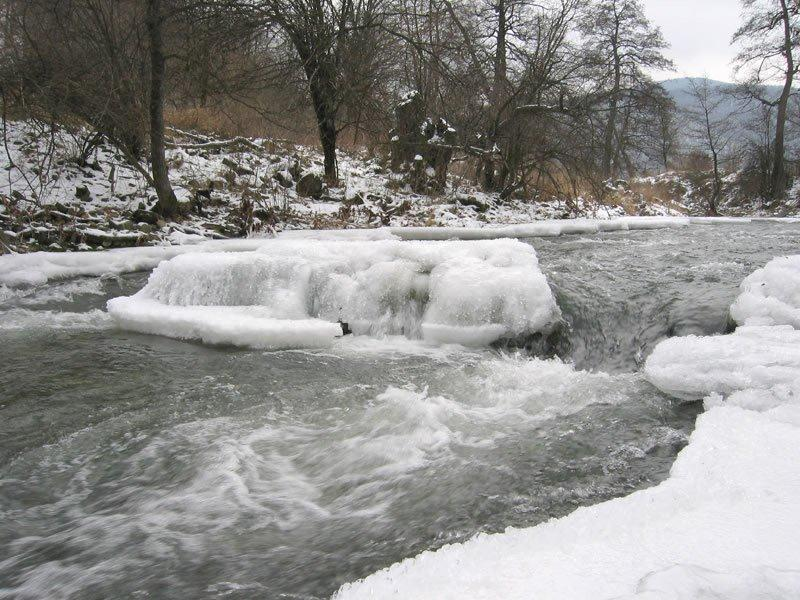
\includegraphics[width=4.5in]{January}\\
\end{figure}

\begin{center}
\textcolor[rgb]{0.00,0.00,1.00}{\\Ask Yourself ...}
\textcolor[rgb]{1.00,0.00,0.00}{\\Who is Speaking?\\Who is being spoken to?\\What is being said?\\Are there
any commandments to obey?\\Are there any promises to claim?}
\end{center}

\end{document}
